\documentclass{beamer}
% Use DS9 global theme
\usepackage{../../../../shared/templates/ds9_theme}

% Title page configuration
\title[Friction and Inclined Planes]{PHYS11 CH:5.4}
\subtitle{Static and Kinetic Friction}
\author[Mr. Gullo]{Mr. Gullo}
\date[Nov 2024]{November 2024}

\begin{document}

\frame{\titlepage}

\section{Introduction to Friction}

\begin{frame}
\frametitle{Learning Objectives}
By the end of this lesson, you will be able to:
\pause
\begin{itemize}
    \item Define friction and distinguish between static and kinetic friction
    \pause
    \item Apply friction formulas: $f_s \leq \mu_s N$ and $f_k = \mu_k N$
    \pause
    \item Resolve weight into components on inclined planes
    \pause
    \item Solve problems involving friction on horizontal and inclined surfaces
    \pause
    \item Use free body diagrams with rotated coordinate systems
\end{itemize}
\end{frame}

\begin{frame}
\frametitle{What is Friction?}
\begin{block}{Definition}
\textbf{Friction} is a force that opposes motion or attempted motion between surfaces in contact.
\end{block}
\pause

\vspace{1em}
\textbf{Key characteristics:}
\begin{itemize}
    \item Acts parallel to contact surface
    \pause
    \item Direction: opposes motion (or attempted motion)
    \pause
    \item Magnitude: depends on surface properties and normal force
    \pause
    \item \textbf{Surprising fact}: Independent of contact area!
\end{itemize}
\end{frame}

\begin{frame}
\frametitle{Types of Friction}
\begin{itemize}
    \item \textbf{Static Friction} ($f_s$): Acts on objects at rest
    \begin{itemize}
        \item Variable force: adjusts to prevent motion
        \item Has maximum value: $f_{s,max} = \mu_s N$
    \end{itemize}
    \pause
    
    \vspace{0.5em}
    \item \textbf{Kinetic Friction} ($f_k$): Acts on objects in motion
    \begin{itemize}
        \item Constant force: $f_k = \mu_k N$
        \item Usually less than maximum static friction
        \item Independent of sliding speed
    \end{itemize}
    \pause
    
    \vspace{0.5em}
    \item \textbf{Important relationship}: $f_{s,max} > f_k$ (always!)
\end{itemize}
\end{frame}

\begin{frame}
\frametitle{Friction Behavior Visualization}
\begin{figure}[H]
    \centering
    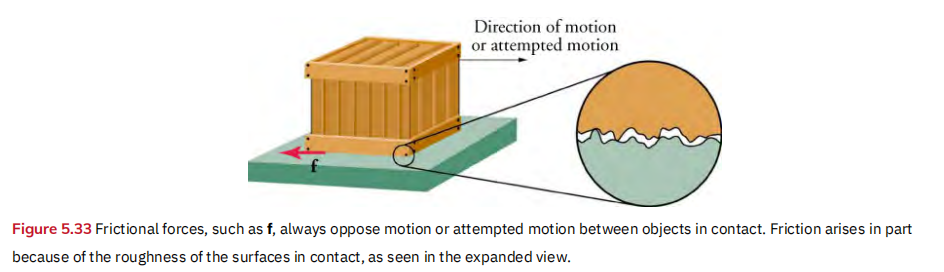
\includegraphics[width=0.8\linewidth]{Screenshot 2024-11-11 110912.png}
\end{figure}

Notice: Static friction increases until maximum, then drops to kinetic friction when motion begins.
\end{frame}

\section{Friction Formulas and Coefficients}

\begin{frame}
\frametitle{Friction Formulas}
\begin{block}{Static Friction}
\[ f_s \leq \mu_s N \]
\textbf{Variables:}
\begin{itemize}
    \item $f_s$ = static friction force (N)
    \item $\mu_s$ = coefficient of static friction (no units)
    \item $N$ = normal force (N)
\end{itemize}
\end{block}
\pause

\begin{block}{Kinetic Friction}
\[ f_k = \mu_k N \]
\textbf{Variables:}
\begin{itemize}
    \item $f_k$ = kinetic friction force (N)
    \item $\mu_k$ = coefficient of kinetic friction (no units)
\end{itemize}
\end{block}
\end{frame}

\begin{frame}
\frametitle{Coefficients of Friction - Real Materials}
\begin{table}
\centering
\begin{tabular}{|l|c|c|}
\hline
\textbf{System} & $\mu_s$ & $\mu_k$ \\
\hline
Rubber on dry concrete & 1.0 & 0.7 \\
Wood on wood & 0.5 & 0.3 \\
Steel on steel (dry) & 0.6 & 0.3 \\
Steel on steel (oiled) & 0.05 & 0.03 \\
Ice on ice & 0.1 & 0.03 \\
\hline
\end{tabular}
\end{table}

\pause
\vspace{0.5em}
\textbf{Observations:}
\begin{itemize}
    \item High friction: rubber on concrete (vehicle safety!)
    \pause
    \item Low friction: ice on ice (explains ice skating)
    \pause
    \item Lubrication effect: oil reduces friction by 10x+
\end{itemize}
\end{frame}

\section{Inclined Planes}

\begin{frame}
\frametitle{Why Study Inclined Planes?}
\textbf{Real-world applications:}
\pause
\begin{itemize}
    \item Skiing and snowboarding
    \pause
    \item Vehicle motion on hills
    \pause
    \item Ramps and accessibility
    \pause
    \item Rock slides and avalanches
\end{itemize}

\vspace{1em}
\pause
\textbf{Key challenge:} Weight acts vertically, but motion is along slope. We need to decompose forces!
\end{frame}

\begin{frame}
\frametitle{Forces on an Inclined Plane}
On a slope at angle $\theta$, weight has two components:
\pause

\begin{block}{Parallel Component (down the slope)}
\[ w_\parallel = mg\sin\theta \]
This component causes motion down the slope.
\end{block}
\pause

\begin{block}{Perpendicular Component (into the slope)}
\[ w_\perp = mg\cos\theta \]
This component is balanced by normal force: $N = mg\cos\theta$
\end{block}
\pause

\vspace{0.5em}
\textbf{Note:} Friction acts parallel to surface, opposing motion: $f = \mu N$
\end{frame}

\begin{frame}
\frametitle{Inclined Plane Force Diagram}
\begin{figure}[H]
    \centering
    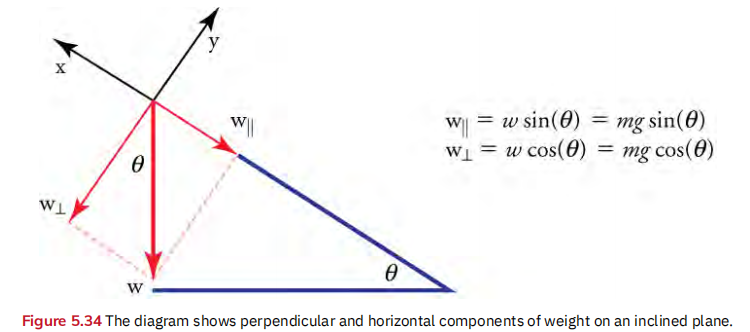
\includegraphics[width=0.7\linewidth]{Screenshot 2024-11-11 110923.png}
\end{figure}

Key: Rotate coordinate system to align with slope direction.
\end{frame}

\begin{frame}
\frametitle{Problem Solving Strategy}
\textbf{Step-by-step approach:}

\begin{enumerate}
    \item Draw sketch of physical situation
    \pause
    \item Identify all known and unknown quantities
    \pause
    \item Draw free body diagram with rotated axes
    \pause
    \item Decompose forces into components
    \pause
    \item Apply Newton's second law:
    \begin{itemize}
        \item If no acceleration: $F_{net} = 0$
        \item If accelerating: $F_{net} = ma$
    \end{itemize}
    \pause
    \item Solve algebraically, then substitute values
    \pause
    \item Check answer for reasonableness (units, magnitude, direction)
\end{enumerate}
\end{frame}

\section{Problem Solving with GUESS Method}

\begin{frame}
\frametitle{Example Problem: Skier on a Slope}
\begin{block}{Problem Statement}
A 62 kg skier slides down a snowy slope inclined at 25°. The kinetic friction force is 45.0 N. Find the coefficient of kinetic friction $\mu_k$.
\end{block}

\begin{figure}[H]
    \centering
    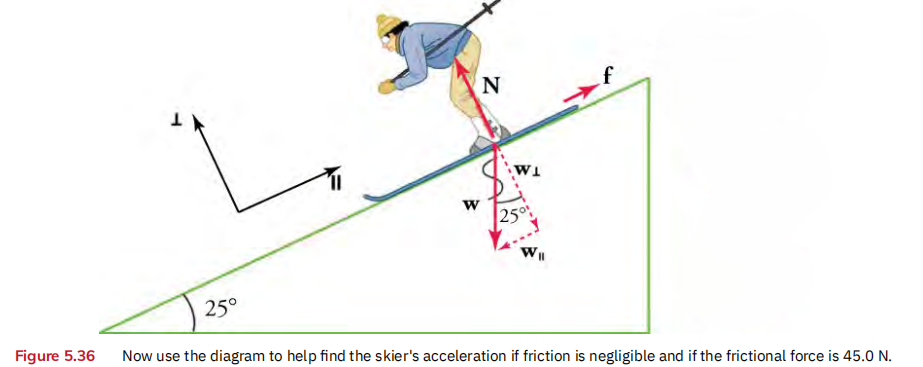
\includegraphics[width=0.7\linewidth]{Screenshot 2024-11-11 110959SansFBD.png}
\end{figure}
\end{frame}

\begin{frame}
\frametitle{Free Body Diagram}
\begin{figure}[H]
    \centering
    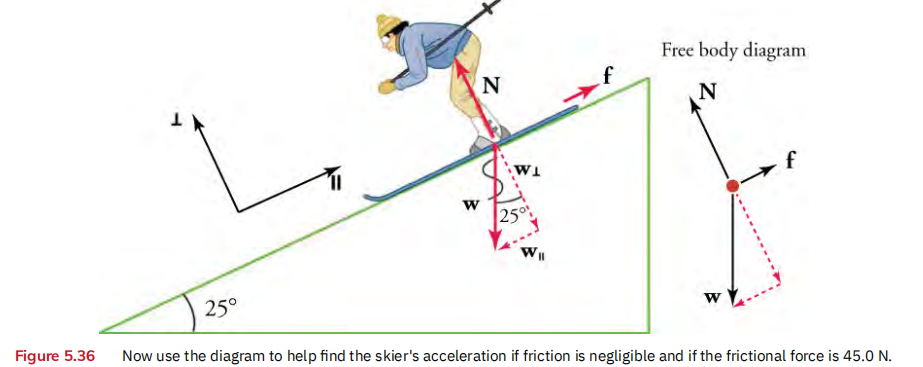
\includegraphics[width=0.9\linewidth]{Screenshot 2024-11-11 110959.png}
\end{figure}

Notice: Axes rotated to align with slope.
\end{frame}

\begin{frame}
\frametitle{Solution: G and U}
\begin{columns}[T]
\column{0.48\textwidth}
\textbf{G - Givens}
\begin{itemize}
    \item $m = 62$ kg
    \item $\theta = 25°$
    \item $f_k = 45.0$ N
    \item $g = 9.80$ m/s²
\end{itemize}

\column{0.48\textwidth}
\textbf{U - Unknown}
\begin{itemize}
    \item $\mu_k = ?$
\end{itemize}
\end{columns}
\end{frame}

\begin{frame}
\frametitle{Solution: E - Equation}
\textbf{E - Equation}

We know: $f_k = \mu_k N$

On incline: $N = mg\cos\theta$

Therefore: $f_k = \mu_k mg\cos\theta$

\textbf{Rearrange for unknown:}
\[ \mu_k = \frac{f_k}{mg\cos\theta} \]
\end{frame}

\begin{frame}
\frametitle{Solution: S - Substitute and Solve}
\textbf{S - Substitute}
\[ \mu_k = \frac{45.0\text{ N}}{(62\text{ kg})(9.80\text{ m/s}^2)\cos(25°)} \]

\pause
\textbf{S - Solve}

First calculate denominator:
\[ N = (62)(9.80)\cos(25°) = 551\text{ N} \]

Then:
\[ \mu_k = \frac{45.0}{551} = 0.082 \]

\vspace{0.5em}
\boxed{\mu_k = 0.082}

\pause
\textbf{Check:} Value is reasonable (between 0 and 1, close to ice on ice).
\end{frame}

\begin{frame}
\frametitle{Example: Acceleration Without Friction}
\begin{block}{Problem - Part A}
What is the skier's acceleration if friction is negligible?
\end{block}

\pause
\textbf{Quick solution:}

Only force down slope: $F = mg\sin\theta$

Apply $F = ma$:
\[ ma = mg\sin\theta \]
\[ a = g\sin\theta \]

\pause
\textbf{Substitute:}
\[ a = (9.80\text{ m/s}^2)\sin(25°) = 4.14\text{ m/s}^2 \]

\boxed{a = 4.14\text{ m/s}^2 \text{ down the slope}}
\end{frame}

\section{Practice Problems}

\begin{frame}
\frametitle{"We Do" Problem: Acceleration with Friction}
\begin{block}{Problem - Part B}
What is the skier's acceleration with 45.0 N friction force?
\end{block}

\pause
\textbf{Setup (together):}

Forces down slope: $F_{down} = mg\sin\theta$

Forces up slope: $F_{up} = f_k$

Net force: $F_{net} = mg\sin\theta - f_k$

\pause
\textbf{You try:} Apply Newton's second law and solve for $a$.

\pause
\textbf{Answer:} $a = 3.39$ m/s² down the slope
\end{frame}

\begin{frame}
\frametitle{"We Do" Solution}
\begin{figure}[H]
    \centering
    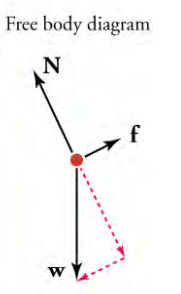
\includegraphics[width=0.2\linewidth]{Screenshot 2024-11-11 111003.png}
\end{figure}

\textbf{Complete solution:}
\[ F_{net} = mg\sin\theta - f_k = ma \]
\[ a = g\sin\theta - \frac{f_k}{m} \]
\[ a = (9.80)\sin(25°) - \frac{45.0}{62} \]
\[ a = 4.14 - 0.73 = 3.41\text{ m/s}^2 \]

\textbf{Observation:} Friction reduces acceleration by about 18\%.
\end{frame}

\begin{frame}
\frametitle{"You Do" Problem}
\begin{block}{Independent Practice}
A 5.0 kg wooden block rests on a wooden incline. The coefficient of static friction is $\mu_s = 0.5$.

\vspace{0.5em}
\textbf{Find:} The maximum angle $\theta_{max}$ before the block starts to slide.

\vspace{0.5em}
\textbf{Hint:} At maximum angle, static friction equals its maximum value and net force is zero.
\end{block}

\vspace{1em}
\pause
\textbf{Try this on your own!} Use the GUESS method.
\end{frame}

\section{Summary}

\begin{frame}
\frametitle{Key Takeaways}
\textbf{Friction concepts:}
\begin{itemize}
    \item Static friction: variable, maximum $f_s \leq \mu_s N$
    \pause
    \item Kinetic friction: constant, $f_k = \mu_k N$
    \pause
    \item Always: $\mu_s > \mu_k$ (harder to start than to keep moving)
\end{itemize}

\pause
\vspace{0.5em}
\textbf{Inclined planes:}
\begin{itemize}
    \item Parallel component: $w_\parallel = mg\sin\theta$ (causes motion)
    \pause
    \item Perpendicular component: $w_\perp = mg\cos\theta$ (balanced by $N$)
    \pause
    \item Friction: $f = \mu N = \mu mg\cos\theta$
\end{itemize}

\pause
\vspace{0.5em}
\textbf{Problem solving:} Use rotated coordinate system and GUESS method!
\end{frame}

\begin{frame}
\frametitle{Friction Force vs Applied Force}
\begin{figure}[H]
    \centering
    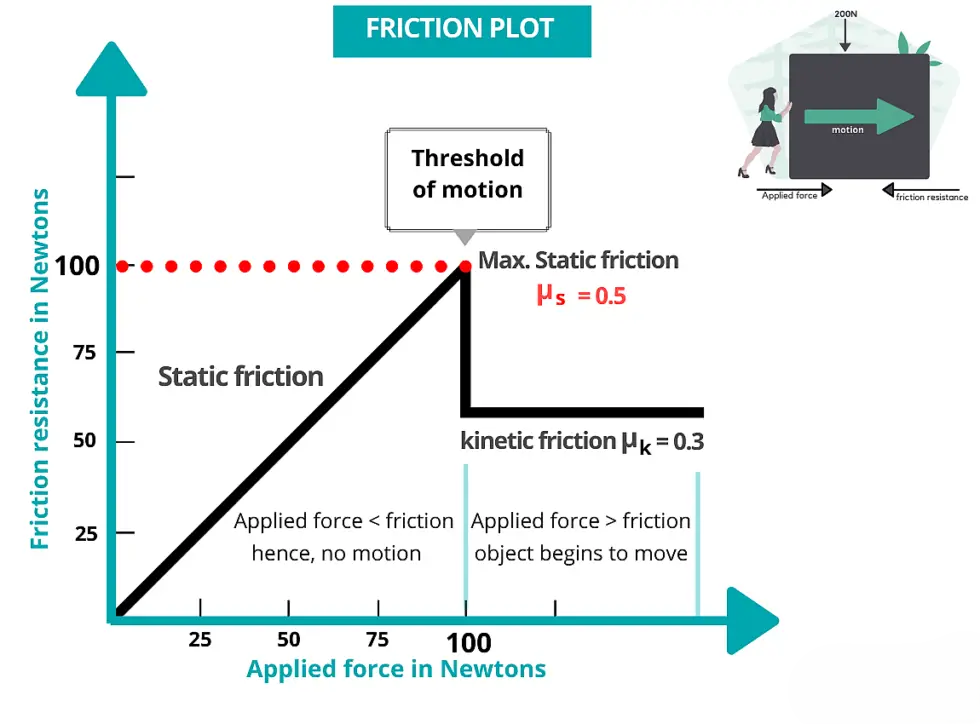
\includegraphics[width=0.9\linewidth]{Friction-Plot-980x724.png}
\end{figure}

\textbf{Remember:} Static friction increases until maximum, then drops to kinetic friction when motion begins.
\end{frame}

\end{document}